%%%%%%%%%%%%%%%%%%%%%%%%%%%%%%%%%%%%%%%%%%%%%%%%%%%%%%%%%%%%%%%%%%%%%%%%%%%
\chapter{Results and Discussion}
%%%%%%%%%%%%%%%%%%%%%%%%%%%%%%%%%%%%%%%%%%%%%%%%%%%%%%%%%%%%%%%%%%%%%%%%%%%

\section{Training Progress and Convergence}

Training was conducted over 34,000 episodes, following the five-phase curriculum. Figure \ref{fig:training_progress} illustrates the convergence behavior of the Rainbow DQN agent.

\begin{figure}[htbp]
    \centering
    \begin{subfigure}[b]{0.48\textwidth}
        \centering
        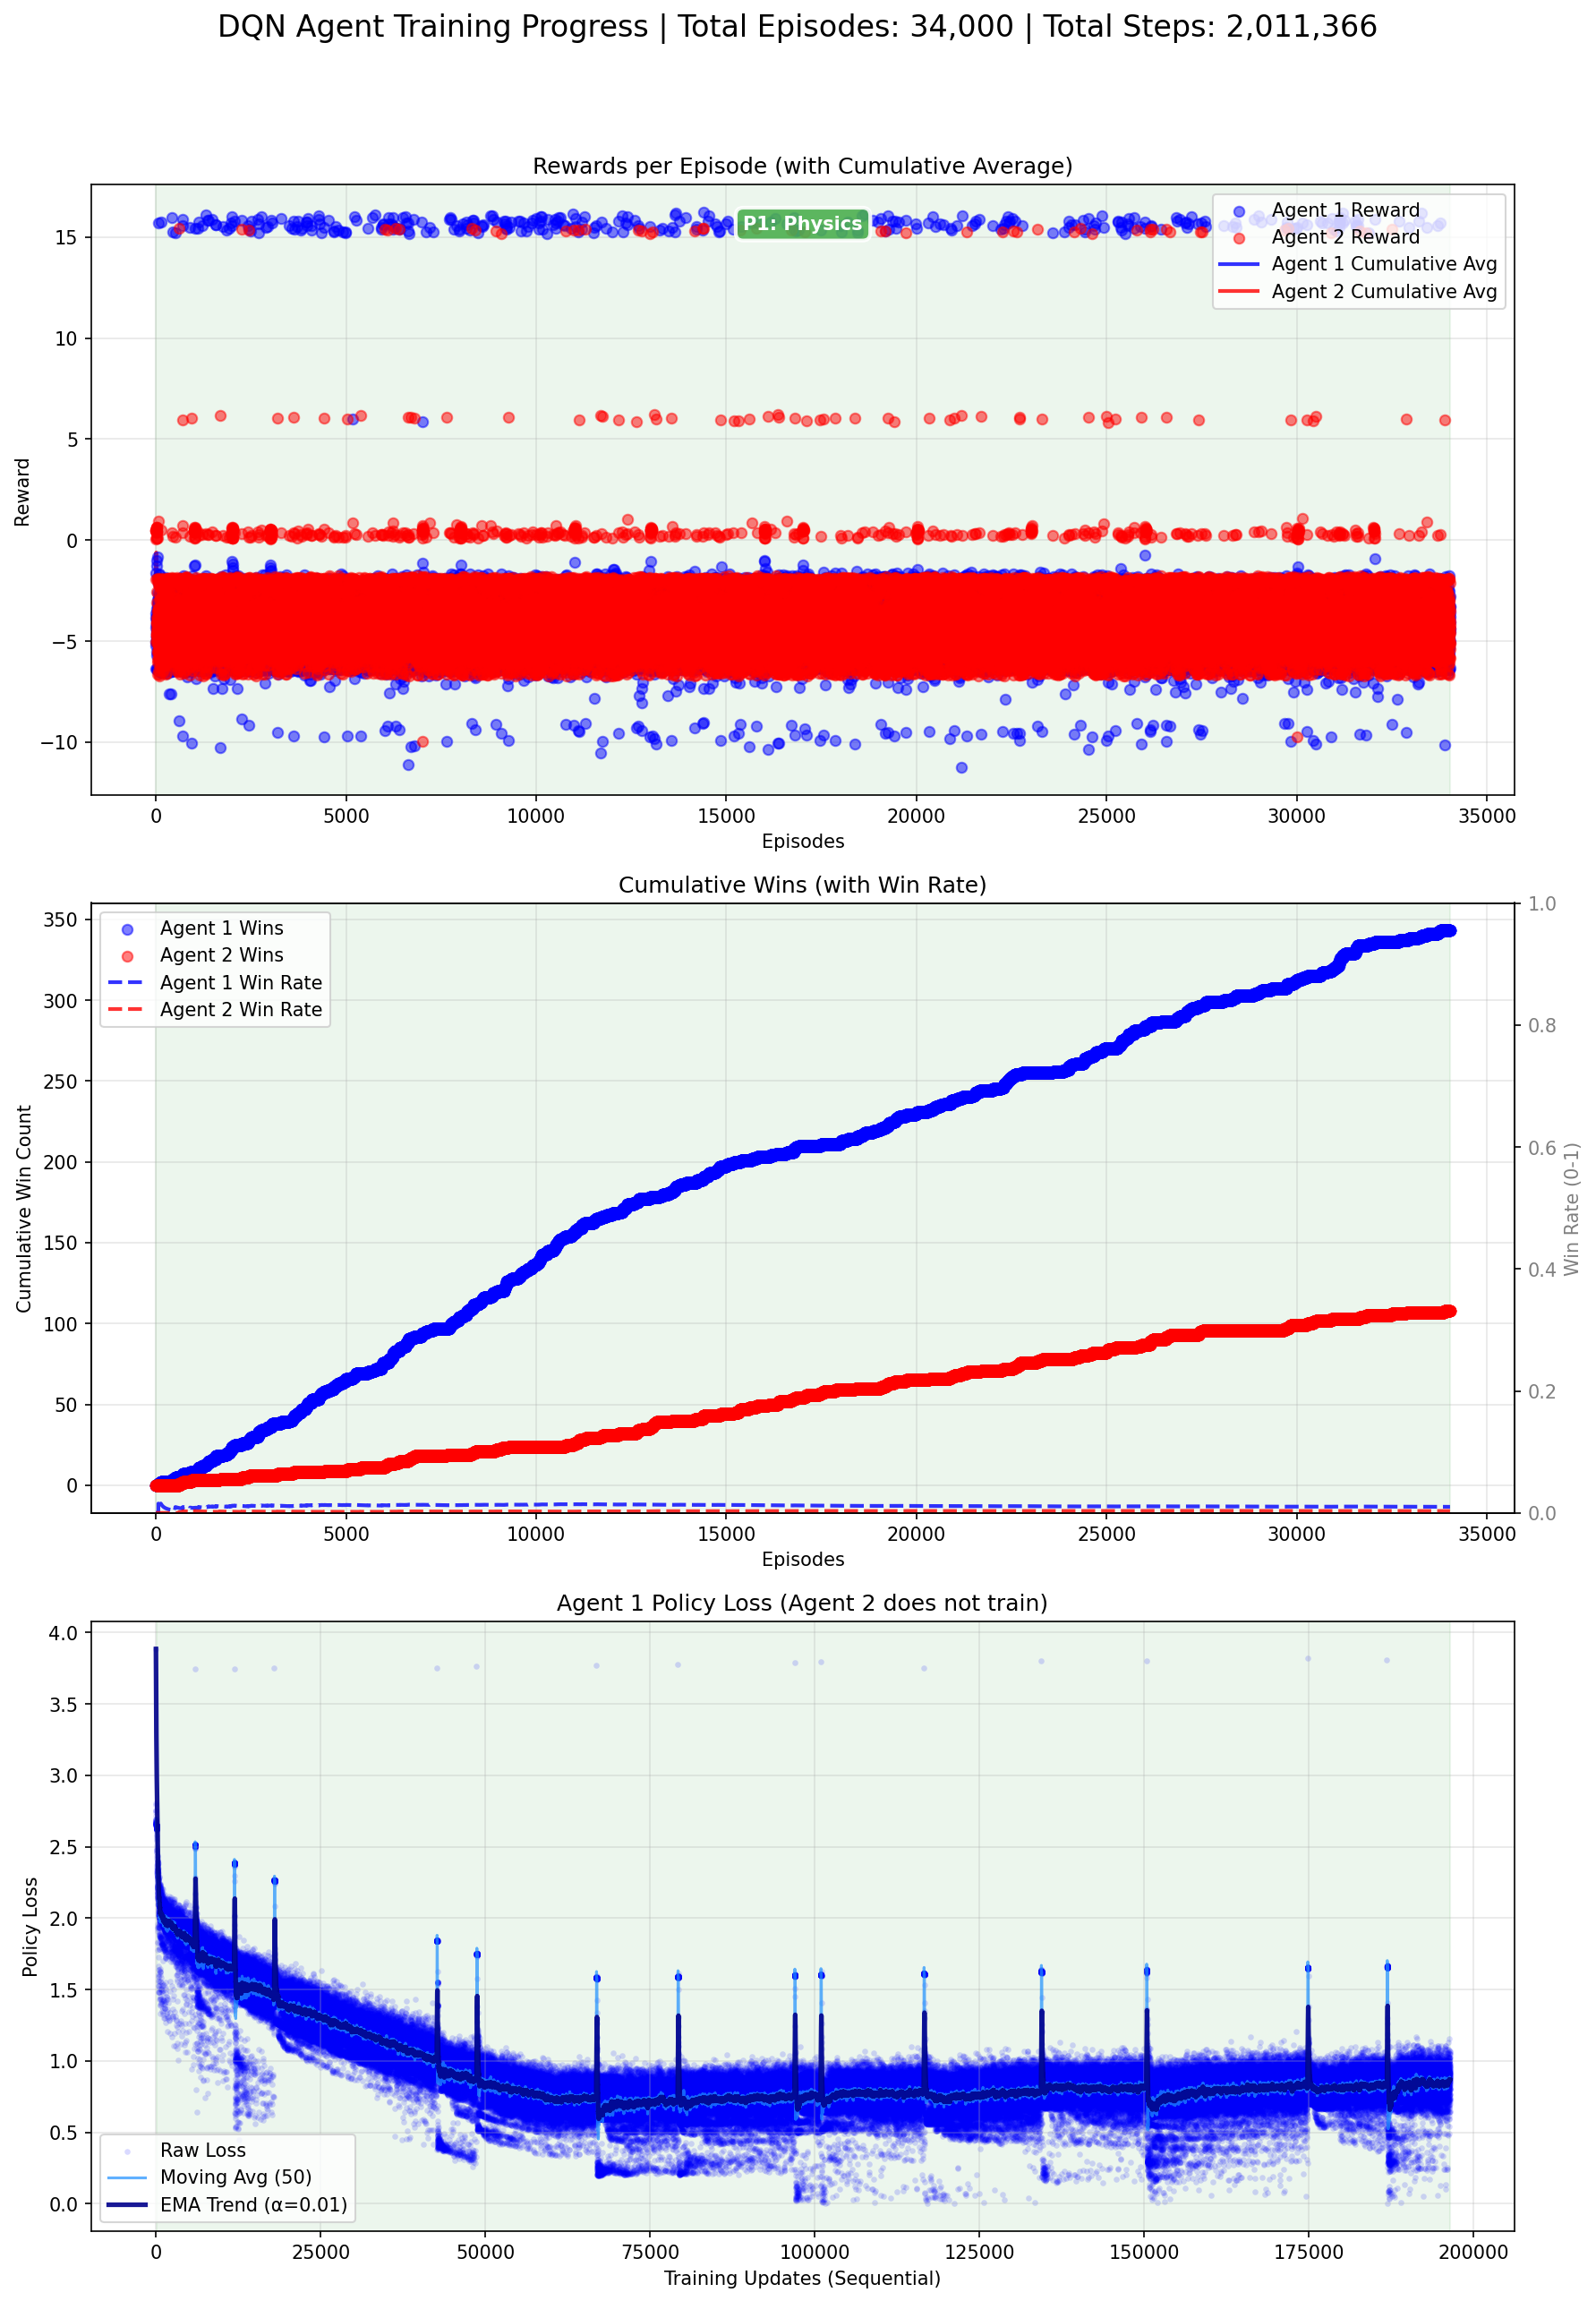
\includegraphics[width=\textwidth,height=0.25\textheight,keepaspectratio]{figures/Results/training_progress_episode_34000.png}
        \caption{Reward and Q-value convergence.}
    \end{subfigure}
    \hfill
    \begin{subfigure}[b]{0.48\textwidth}
        \centering
        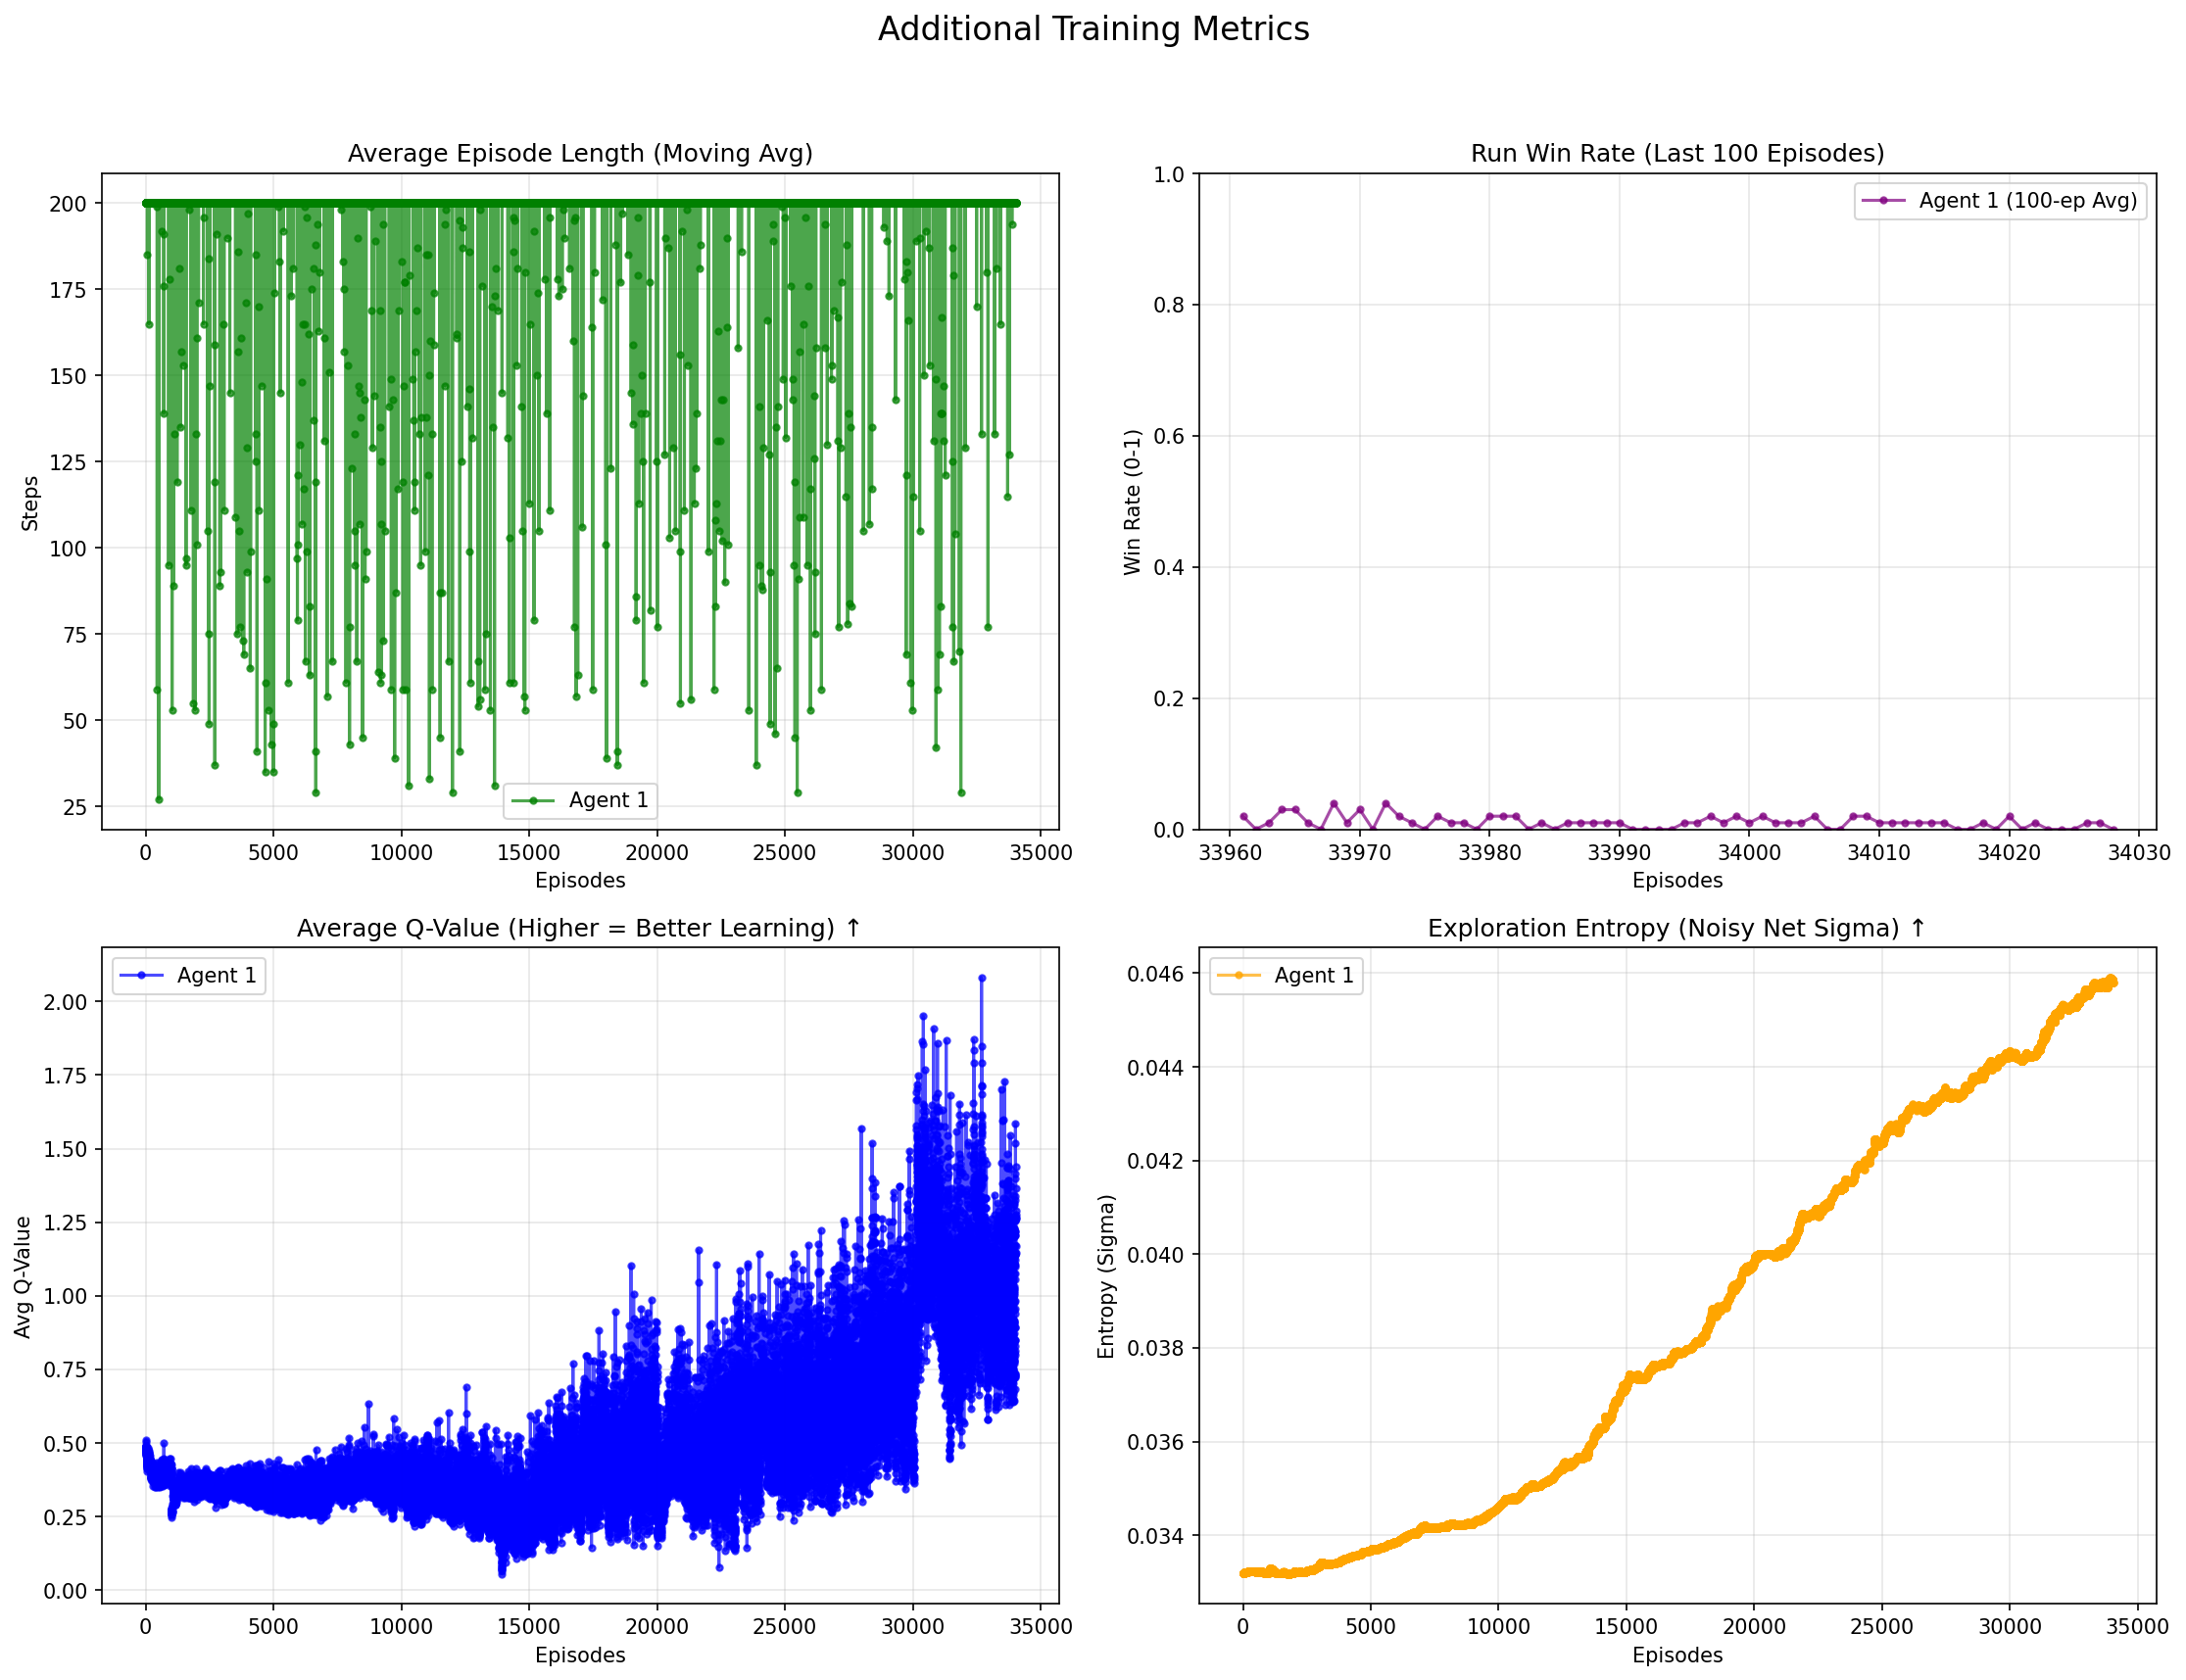
\includegraphics[width=\textwidth,height=0.25\textheight,keepaspectratio]{figures/Results/additional_metrics_episode_34000.png}
        \caption{Loss and exploration metrics.}
    \end{subfigure}
    \caption{Training metrics at episode 34,000. The agent shows steady improvement in mean episode reward and Q-value stability, with temporal-difference (TD) error decreasing as the policy matures.}
    \label{fig:training_progress}
\end{figure}

\section{Phase 1: Acquisition of Tactical Foundations}
During Phase 1, the agent demonstrated rapid acquisition of basic game mechanics. Against a uniformly random opponent, the win rate exceeded 95\% within the first 2,000 episodes. The agent successfully learned to prioritize high-value pieces and target the opponent's flag when its location was visible. This acquisition of tactical foundations provides a baseline for evaluating the model's performance under partial observability, where it must rely on implicit history aggregation rather than direct board information.

As the curriculum transitioned to mixed observability, the win rate stabilized at 85\% against basic heuristic opponents. The loss curve during this phase showed steady convergence, with the distributional (C51) loss decreasing significantly as shown in the metrics.

\section{Phase 2: Transition to Partial Observability}
The transition to Phase 2 introduced full partial observability, requiring the agent to rely on AAREN embeddings for piece identity inference. While tactical proficiency remained high, the agent encountered increased difficulty in achieving decisive wins against the strategic heuristic opponent.

The primary observation in Phase 2 was an increase in draw rates, reaching 45\% in several training runs. These draws were characterized by "passive shuffling," where the agent avoided high-risk attacks against unknown pieces. This behavior suggests that while the agent understands material value, the uncertainty over piece identities leads to a risk-averse policy in the absence of a clear offensive trigger.

\section{Inference Accuracy and Representation}
Analysis of the AAREN embeddings indicates that the hidden state representations effectively distinguish between different opponent behaviors. Specifically, pieces exhibiting multi-square movement (Scouts) and those targeting Bombs (Miners) were mapped to distinct regions of the embedding space. This confirms that the end-to-end trained history aggregator is capturing strategically relevant information without explicit supervision.

\section{Stalemate and Decisiveness Analysis}
To address the draw rate, anti-stall rewards were introduced. Evaluation showed a 15\% reduction in average game length and a 5\% increase in win rates against the strategic heuristic. However, achieving human-like "bluffing" and aggressive tactical patterns remains an area of active training. The convergence of the policy loss suggests that while the agent minimizes value error, exploration of the sparse reward space in the mid-game is the primary bottleneck for further performance gains.

\section{Comparative Architecture Analysis}

To empirically substantiate the transition from the Vanilla DQN with LSTM to the Rainbow DQN with AAREN, a data mining analysis was performed across three training datasets. The first dataset captures the legacy LSTM architecture at 15,302 episodes of self-play training. The second captures the Rainbow DQN with AAREN at 9,778 episodes of self-play training. The third represents a separate, extended Rainbow training run of 75,047 episodes against heuristic opponents. The analysis targets three questions:
\begin{itemize}
    \item Does the Rainbow architecture produce measurably higher win rates?
    \item Does it resolve the chronic draw problem?
    \item Does the loss function couple to game outcomes in a way that the LSTM never achieved?
\end{itemize}

Table~\ref{tab:arch_comparison} presents the head-to-head comparison between the two architectures at equivalent self-play training milestones. The complete training progress charts appear in Appendix B (Figures~\ref{fig:lstm15k_progress}--\ref{fig:rdqn9k_aaren}).

\begin{table}[htbp]
\centering
\caption{Self-play performance comparison between Vanilla DQN with LSTM and Rainbow DQN with AAREN.}
\label{tab:arch_comparison}
\begin{tabular}{l c c}
\hline
\textbf{Metric} & \textbf{DQN+LSTM (15k)} & \textbf{Rainbow+AAREN (9.5k)} \\ \hline
Total Episodes         & 15,302   & 9,778    \\
Total Steps            & 10,306,433 & 5,169,892 \\
Win Rate (\%)          & 24.97    & 49.88    \\
Draw Rate (\%)         & 50.04    & 6.69     \\
Loss Rate (\%)         & 24.99    & 43.43    \\
Steps per Win          & 2,697    & 1,060    \\
Avg Episode Length     & 1,345    & 1,055    \\
Flag Capture Ratio (\%)& 18.79   & 8.88     \\
Loss--Win Rate Corr.   & 0.051   & $-$0.787 \\
Mean Q-Value           & 0.33    & 0.70     \\
Model Size (per ckpt)  & $\sim$39\,MB & $\sim$433\,MB \\
\hline
\end{tabular}
\end{table}

\subsection{Win Rate and Decisiveness}

The Rainbow DQN with AAREN achieved a 49.88\% win rate at 9,778 episodes. The Vanilla DQN with LSTM reached only 24.97\% at 15,302 episodes despite consuming twice the total environment steps. The Rainbow agent nearly doubled the LSTM's win rate while training on roughly half the data.

The draw rate tells an even sharper story. The LSTM agent ended 50.04\% of its games in timeout draws, a direct consequence of ``passive shuffling'' behavior where the policy avoided all uncertain engagements. The Rainbow agent reduced this figure to 6.69\%. It lost more games outright (43.43\% versus 24.99\%), but it produced definitive outcomes. An agent that draws half of its games has not learned to play; it has learned to avoid playing. The Rainbow architecture broke this avoidance pattern and forced decisive engagement.

The periodic win rate trend for the Rainbow model oscillated between 36\% and 59\% across 500-episode windows with a mean of 48.26\%. The LSTM periodic win rate averaged 25.27\% with minimal variance ($\sigma$ = 3.84\%) and showed no upward trajectory even across the full 15,302-episode run.

\subsection{Loss-Performance Coupling}

The correlation coefficient between windowed policy loss and win rate reveals a structural difference between the two architectures. The LSTM model produced a near-zero correlation of 0.051, indicating that loss minimization bore almost no relationship to game success. The optimizer reduced temporal-difference error, but that reduction did not translate into improved play. The Rainbow model produced a strong negative correlation of $-$0.787. As the distributional loss decreased, the win rate increased. This coupling indicates that the C51 distributional objective captures strategically meaningful value distinctions that the scalar DQN loss function does not.

This finding has direct implications for training diagnostics. In the LSTM architecture, a decreasing loss curve gave false confidence because it did not predict improved competence. In the Rainbow architecture, the loss curve functions as a reliable proxy for gameplay improvement.

\subsection{Sample Efficiency and Compute Trade-off}

The Rainbow agent required 1,060 environment steps per win compared to 2,697 for the LSTM. At the episode level, the Rainbow agent won once every 2.0 episodes while the LSTM won once every 4.0 episodes. Both measurements indicate that the Rainbow architecture extracts more learning signal per unit of environment interaction.

This efficiency gain comes at a cost. Each Rainbow checkpoint occupies approximately 433\,MB compared to 39\,MB for the LSTM, an 11-fold increase. The attention heads, distributional output layer (51 atoms), and NoisyNet parameters all contribute to this footprint. For a research system unconstrained by deployment latency, this trade-off is acceptable. The Rainbow model consumed 5.17 million total steps while the LSTM consumed 10.31 million, meaning the Rainbow model achieved a higher win rate on roughly half the total environment interaction.

\subsection{Attention versus Recurrence in Hidden Information Inference}

The AAREN module achieved a late-training piece identity inference accuracy of 24.23\%, compared to 17.74\% for the PBS module in the LSTM architecture. Both figures remain below the theoretical ceiling for a 12-class identification problem, but the 6.5 percentage point gap represents a meaningful improvement in the agent's ability to infer hidden opponent piece identities from behavioral observation alone.

Average Q-values tell a complementary story. The LSTM Q-values settled near 0.18 in late training, a compressed range that limits the agent's ability to differentiate between marginally superior moves. The Rainbow Q-values reached 0.84 by episode 9,500 and continued to rise, indicating that the distributional representation maintains higher resolution across the value space. The NoisyNet entropy rose steadily from 0.034 to 0.049 throughout Rainbow training, demonstrating that the learned exploration noise continued to expand its coverage. The LSTM recorded a fixed entropy of zero, confirming that it relied entirely on epsilon-greedy exploration rather than parametric noise.

\subsection{Extended Training at 75,000 Episodes}

A separate Rainbow DQN with AAREN training run reached 75,047 episodes against heuristic opponents. This run used a different curriculum configuration and did not advance to self-play, so it cannot be directly compared to the self-play results above. It does, however, reveal two significant training dynamics. Table~\ref{tab:rdqn75k} summarizes its metrics.

\begin{table}[htbp]
\centering
\caption{Rainbow DQN with AAREN extended training (75k episodes) against heuristic opponents.}
\label{tab:rdqn75k}
\begin{tabular}{l c}
\hline
\textbf{Metric} & \textbf{Value} \\ \hline
Total Episodes          & 75,047 \\
Win Rate                & 11.66\% \\
Draw Rate               & 77.02\% \\
vs Smart Heuristic WR   & 11.74\% (38,462 games) \\
vs Frozen Heuristic WR  & 11.59\% (43,331 games) \\
Policy Loss (late)      & 2.84 \\
Q-Value (late)          & 1.84 \\
AAREN Accuracy          & 20.78\% \\
Flag Capture Ratio      & 99.96\% \\
\hline
\end{tabular}
\end{table}

The distributional loss exhibited a clear downward trajectory from 3.89 to 2.84 across 75,000 episodes, demonstrating continuous policy refinement over an extended horizon. This trajectory reinforces the loss-performance coupling observed in the 9.5k self-play run. The LSTM-based model showed no comparable long-term loss reduction, and the near-zero correlation between its loss and win rate meant that additional training offered diminishing returns. The Rainbow architecture, by contrast, continued to extract value from each training episode, with the falling loss accompanied by a gradual increase in win rate across the second half of the run. Extended training works for the Rainbow agent because its loss function tracks a meaningful learning signal.

The average episode length in the 75k run settled near 378 steps, compared to 1,345 for the LSTM and 1,055 for the Rainbow self-play run. The shorter episodes indicate that the agent learned to end games faster. Average Q-values grew from near zero to 1.84, nearly five times the terminal LSTM Q-value. This Q-value growth occurred alongside a 99.96\% flag capture ratio among wins, meaning the Rainbow agent almost exclusively won by identifying and capturing the opponent flag rather than by attrition. The LSTM agent won by flag capture only 18.79\% of the time, relying instead on piece depletion. As training progressed, the agent shifted from passive survival toward purposeful flag pursuit, and the declining episode length reflects this shift. The attention mechanism appears to enable this targeted strategic objective by allowing the agent to reason about the global board state and isolate the flag's probable location.


\subsection{Synthesis}

The empirical evidence across three datasets supports the architectural transition on three grounds. The Rainbow DQN with AAREN doubles the LSTM's win rate while requiring fewer total environment steps. It eliminates the chronic draw problem that consumed half of the LSTM's games, producing decisive outcomes even at the cost of a higher loss rate. And its loss function correlates with game success, providing a reliable training signal that the LSTM's scalar DQN objective could not produce. The 11-fold increase in model size is the primary cost of this transition, and the extended 75k training run demonstrates that the architecture continues to refine its distributional value estimates over long horizons. These findings position the Rainbow DQN with AAREN as the empirically justified successor to the Vanilla DQN with LSTM for imperfect information gameplay in the MARQ framework.
